\documentclass{article}

%\usepackage{loubookman}
\usepackage{loustandard}
\usepackage{graphics}
\usepackage[tt]{codedocn}


\newcommand{\OsiTwo}{OSI2\xspace}
\newcommand{\revisionDate}{September 29, 2011}

\begin{document}
\markright{\OsiTwo \hfil Design and Architecture \hfil \revisionDate}

\heading{\OsiTwo Design and Architecture}

This document describes the design and architecture plans for \OsiTwo.

There are a number of overarching goals:
\begin{itemize}
  \item
  A plugin API architecture, so that individual APIs can be kept to a
  manageable size and implementation of a module in support of
  an API is a manageable task.

  \item
  Dynamic loading of solvers and other functional modules in support of
  specific APIs.

  \item
  An implementation that is primarily a lightweight and (when necessary)
  transparent plugin management layer.
\end{itemize}
This leads to a use model where clients create an \OsiTwo object and then
request it to load modules (often, but not necessarily, solvers) that
implement specific APIs.
In response to a request,
the \OsiTwo object loads the requested module, invokes the module's factory
methods to produce an object supporting the requested API(s), and hands this
object over to the client.
Clients interact with these objects according to the definition of the API\@.

The \OsiTwo object acts as a broker, handling the mechanics of managing 
the plugins.

\subheading{Plugin Architecture}

The plugin architecture used in \OsiTwo is broadly adopted from an
architecture originally described by G.~Sayfan \cite{say07}.

There is one (static) instance of the plugin manager, returned by a call to
\pgmid{getInstance}.
The plugin manager provides certain services and information to plugins,
defined by the \pgmid{PlatformServices} class.
In particular, a \pgmid{PlatformServices} object specifies a registration
method that allows a plugin to register with the plugin manager, and it
provides a service method that the plugin can invoke to request other
services from the manager (currently unimplemented).

An immediate deficiency in the original architecture is that the plugins used
for \OsiTwo are in general not stateless, hence the architecture has been
expanded
to allow a reference to a plugin object to be returned to the plugin manager
and passed back whenever plugin services are invoked.

The working sequence to load a plugin and return an object to the client is
described below.
The first two steps (loading the shared library, initialising the plugin and
registering APIs) are encapsulated in \pgmid{PluginManager::loadOneLib}, so
that load and initialisation of a plugin library is an atomic action from the
point of view of a client of the plugin manager.
\begin{enumerate}
  \item
  Load the shared library that implements the plugin.

  Currently, this is accomplished by a call to the static \pgmid{load}
  method in the \pgmid{DynamicLibrary} class.
  The plugin manager supports specification of a default plugin directory.
  \aside{We need to add infrastructure to check the environment. We might also
  want to allow for a search list of directories.}

  \item
  Initialise the plugin library and register APIs implemented the library.

  Given a \pgmid{DynamicLibrary} object, \pgmid{getSymbol} is used to
  retrieve the plugin library's \pgmid{initPlugin} method.
  This method is then invoked,
  passing a \pgmid{PlatformServices} structure as a parameter.

  The \pgmid{initPlugin} method is responsible for getting the plugin ready to
  work and registering its capabilities (APIs).
  (For example, the \pgmid{ClpShim} plugin is responsible for loading the clp
  solver library.)
  For each API supported by the plugin library, a
  \pgmid{RegisterParams} object
  is created specifying an identifying string, create and destroy methods,
  descriptive information (version and language), and an associated
  object to hold any state information the plugin wishes to maintain for
  objects supporting this API.
  The \pgmid{RegisterParams} object is handed back to the plugin manager
  as a parameter to the registration (\pgmid{registerObject}) method
  supplied in the \pgmid{PlatformServices} object.

  The plugin manager's \pgmid{registerObject} method adds the
  \pgmid{RegisterParams} object to an appropriate temporary structure
  (exact match or wildcard) according to the identifying string.
  It then returns to the \pgmid{initPlugin} method.

  The \pgmid{initPlugin} method returns an appropriate cleanup method (an
  \pgmid{ExitFunc}) when it returns to the plugin manager.
  The plugin manager stores it for use when the plugin library is unloaded.
  Initialisation is complete.
  \aside{Currently there are multiple structures in the plugin manager holding
  information about a plugin, and they are not correlated~---~for example,
  it's not possible to identify the library associated with an exit function.
  This should be fixed.}

  \item
  Ask the plugin manager for an object that implements an API.

  Using the plugin manager's \pgmid{createObject} method, the user asks for an
  API by name.
  The \pgmid{createObject} method searches the maps held by the plugin manager
  looking for a suitable match.
  An \pgmid{ObjectParams} object is created, including the API(s) requested, a
  \pgmid{PlatformServices} object, and the plugin object itself (the only way
  for the plugin to maintain state across calls).
  This is passed as a parameter to the create function that the plugin
  registered for this type of API.
  The returned object is handed back to the client.
\end{enumerate}

It's useful to note that a given plugin library (loadable shared library)
can supply multiple APIs, and asking for an object that implements some
combination of APIs is possible.
It's the business of the plugin object to keep track of what particular APIs
or combination of APIs it supports, and what objects it's given out.

Which begs the question, ``How will the plugin manage capabilities?''
I guess in the end it's the plugin's problem.
If it hands out a single object that supports some number of APIs, then
there's no real issue.
If it can do more complicated things, then it'll need a way to handle that.

On our side, perhaps some sort of \pgmid{inquireAPI} method that'll
allow the plugin to inspect an API and decide if it supports it.

And now I can see an interesting issue.
The client asks for some set of APIs.
It could well be that the client has loaded more than one plugin capable of
supporting the API set.
Some solvers are better at one task, some at another.
Do we allow the user to choose?
Seems like we have to.

And what about that plugin that hands out a single object that supports
multiple APIs?
How (should?) we allow the client to signal that it wants the same object, if
possible.
In the opposite case, the client might want an entirely clean object, not
connected with the previous one even when that's possible.



\subheading{API Architecture}

APIs will derive from a common top-level virtual class \pgmid{Osi2::API} as
shown in Figure~\ref{fig:OsiTwoAPIHierarchy}.
\begin{figure}[b]
\begin{center}
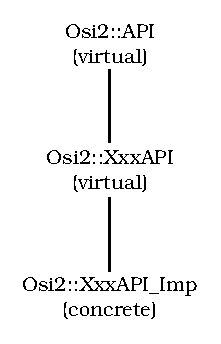
\includegraphics{apihierarchy}
\end{center}
\caption{Class Hierarchy for Osi2 APIs}
\label{fig:OsiTwoAPIHierarchy}
\end{figure}

\bibliographystyle{plain}
\bibliography{osi2design}

\end{document}

